\section{Validating SimCADO by modelling the VLT/HAWK-I optical system}
\label{sec:hawki}

Aside from testing during the coding phase, we tested the accuracy of SimCADO by comparing simulated raw detector readout images to raw observations from HAWK-I on UT4 at the VLT. HAWK-I, the High Acuity Wide-field K-band Imager \citep{hawki}, is a present-day analogue to MICADO's imaging modes and thus a good test-bed for these comparisons. In order to create a version of SimCADO that simulates raw observations for the VLT/HAWK-I optical train, we created a simulation configuration file that reflects the UT4/HAWK-I optical train from the publicly available instrument data on the ESO website\footnote{\url{http://www.eso.org/sci/facilities/paranal/instruments/HAWK-I.html}} and from HAWK-I calibration data from the ESO archive. The verification process included two tests on the simulated output data. The first tested whether the HAWK-I version of SimCADO could reproduce the sensitivity limits of the VLT/HAWK-I system as given in \citet{hawki}. The second involved simulating images of two globular clusters and comparing them against the real images from the ESO archive. The raw images used for the comparison were several J and Ks images of the globular clusters M\,4 and NGC\,4147, downloaded from the ESO archive.

\subsection{Modelling HAWK-I with SimCADO}

To create a model of the HAWK-I optical train, SimCADO required the following data:
\begin{itemize}
    \item an estimate of the Point Spread Function (PSF) for the whole VLT/HAWK-I system,
    \item transmission/reflectivity curves for each of the surfaces along the optical path, 
    \item details of the HAWAII-2RG detector characteristics
\end{itemize}

Additionally, a description of the globular clusters to be observed was needed. Creating the descriptions of the on-sky sources is described in more detail in Sect.~\ref{subsec:HAWKI_comparison}.

\paragraph{The point spread function (PSF):}
The seeing-limited nature of the UT4/HAWK-I optical train greatly simplified simulations. The combined system PSF can be described by a diffraction limited Moffat profile for the round monolithic mirrors of the UT4 telescope \citep{vlt_mirror} combined with a Gaussian profile for the atmospheric contribution. We used the POPPY package \citep{poppy} to generate a diffraction limited PSF for an 8.2\,m circular aperture with a 1.1\,m secondary obscuration and four support beams with a width of 0.1\,m. We then convolved this diffraction-limited PSF with a $0.5\arcsec$ 2D Gaussian profile to mimic the seeing-limited nature of HAWK-I observations. This artificial PSF can be seen in the bright stars in the right image of Fig.~\ref{fig:img_comparison}.

\paragraph{Transmission curves for the optical train:}
The combined optical train of HAWK-I and the VLT's UT4 contains 7 aluminium-coated mirrors, an entrance window, a series of standard NIR filters and a detector plane with four~HAWAII-2RG detectors. The transmission, reflectivity and quantum efficiency curves for each of these elements were combined in SimCADO. The resulting transmission curve has an average transmission value of 0.52, which is very similar to the average value of 0.5 assumed by the online exposure time calculator provided by ESO.\footnote{\url{https://www.eso.org/observing/etc/bin/simu/HAWK-I}}

\paragraph{The detector array:}
Four HAWAII-2RG detectors \citep{hawaii2rg} make up the HAWK-I detector plane. The detector noise was generated internally by SimCADO using the NGHxRG package \citep{nghxrg}. The quantum efficiency curve was taken from \citet{finger2008}. The detector linearity curve was extracted from the Ks-band archive image \verb+HAWK-I.2015-06-10T05_12_28.683+. It was determined by fitting Gaussian profiles to the wings of a series of saturated stars in the raw observations and comparing the theoretical height of the best-fit Gaussian profile to the actual pixel values in saturated regions. The plate scale used by SimCADO was $0.106\arcsec$, as reported by \citet{hawki}.

%Instrumental distortion was neglected because its effect was minimal when determining the photometric accuracy of a simulated stellar field. 
The flat field effect of the whole system was neglected for these tests. The archive images were not flat field corrected, and no flat field was applied to the simulated images. This decision was made because the vast majority of the stars in the globular clusters were located in the central region of the image where the variable field illumination plays a negligible role with respect to the photometric accuracy.

%It should be noted that we are in the process of conducting a further study to quantify the extent to which different atmospheric conditions affect the accuracy of images generated with SimCADO. For this study we were granted 5~hours of technical time on HAWK-I and will report on the results in a future paper. 


\subsection{Test 1 - HAWK-I Sensitivity with SimCADO}

\begin{table}
    \centering
    \caption{Limiting Vega magnitudes calculated for HAWK-I from images generated by SimCADO, the ESO ETC and taken from \citet{hawki}. The SimCADO limiting magnitudes were calculated based on a $5\sigma$ detection in a grid of 100 stars with magnitudes spread linearly between 14\m and 27\m in the respective filters. The FWHM for the SimCADO PSF was chosen to match the ``Image Quality'' parameter given by the ETC. For a seeing value of $0.8\arcsec$ in V band and an airmass of 1.2, the resulting FWHM for J, H, and Ks (\brgamma) band respectively was $0.62\arcsec$, $0.58\arcsec$, $0.53\arcsec$.}
    \label{tab:HAWKI_lim_mags}
    \begin{tabular}{ l  r r r r }
    \hline\hline
    Filter & Exposure  & SimCADO          & ETC                &  KP+2008 \\
           &           & (Vega)           & (Vega)            & (Vega)  \\
    \hline
           & 1 hr           &  23.8\m          &  24.2\m            &  23.9\m          \\
    J      & 1 min          &  21.5\m          &  22.0\m            &                    \\
           & 2 sec          &  19.7\m          &  20.1\m            &                    \\
    \hline
           & 1 hr           &  22.7\m          &  23.3\m            &  22.5\m          \\
     H     & 1 min          &  20.5\m          &  21.0\m            &                    \\
           & 2 sec          &  18.8\m          &  19.2\m            &                    \\
    \hline
           & 1 hr           &  21.9\m          &  22.2\m            &  22.3\m          \\
    Ks     & 1 min          &  19.7\m          &  19.9\m            &                    \\
           & 2 sec          &  17.8\m          &  18.1\m            &                    \\
    \hline
   	       & 1 hr           &  21.6\m          &  20.9\m            &                    \\
\brgamma   & 1 min          &  19.5\m          &  18.7\m            &                    \\
           & 2 sec          &  17.5\m          &  16.8\m            &                    \\
    \hline
    \end{tabular}

\end{table}

As a first test we compared the limiting magnitudes of images generated with SimCADO to both the limiting magnitudes given by \citet{hawki}, and those given by the exposure time calculator (ETC) on the ESO website. For the SimCADO model of HAWK-I we determined the limiting magnitudes by simulating images of a grid of 100 stars with magnitudes ranging from 15\m to 27\m in each of the HAWK-I filters. The grid was ``observed'' for a series of exposure times ranging from 2\,seconds to 1~hour. As the positions of the stars were known, we used aperture photometry to calculate the signal to noise ratio (SNR) for each of the stars in each of the exposure and filters. The limiting magnitude for image was set by the star with a SNR closest to, but not lower than $5\sigma$. The results for various exposure times are shown in Table \ref{tab:HAWKI_lim_mags} and for the J-band in Fig. \ref{fig:HAWKI_rainbow_j}.

It can be seen from Table~\ref{tab:HAWKI_lim_mags} that the limiting magnitudes for SimCADO in the J and H filters are within 0.2\m of the values given by \citet{hawki}, although there is a $\sim$0.5\m discrepency between SimCADO and the ETC. In the Ks filter the discrepancy is only $\sim$0.3\m. The \brgamma filter shows the biggest deviation of $\sim$0.7$\m. The observation parameters used in SimCADO were set to be identical to those described by \citet{hawki}, namely: seeing of $0.8\arcsec$ in V-band and an airmass of 1.2. Fig.~\ref{fig:HAWKI_rainbow_j} shows the evolution of several relevant detection limits (e.g.\ $5\sigma$ for photometry, $\sim 250\sigma$ for astrometry) for HAWK-I as determined by SimCADO.


\begin{figure}

    \centering
    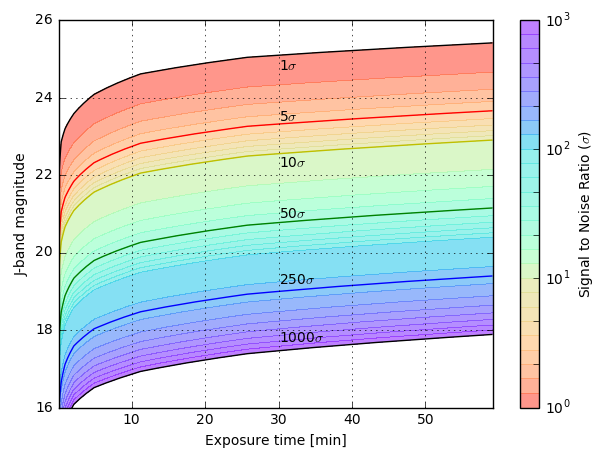
\includegraphics[width=0.48\textwidth]{images/HAWKI_SNR_Rainbow_J}
    
    \caption{Limiting Vega magnitudes as predicted by SimCADO for the UT4/HAWK-I optical system. A grid of hundred stars were observed for different durations between 1 and 60 minutes using SimCADO configured to model UT4/HAWK-I. The $5\sigma$ contour in this graph is $\sim 0.5$\m lower than the theoretical $5\sigma$ detection limits as returned by the ESO HAWK-I ETC. However the one hour $5\sigma$ Vega magnitude limit ($J=23.7$\m) is within 0.2\m  of the limit published by \citet{hawki}.}
    \label{fig:HAWKI_rainbow_j}

\end{figure}


\subsection{Test 2 - Comparison of SimCADO images with real observations}
\label{subsec:HAWKI_comparison}

\begin{table*}

    \centering
    \caption{The raw un-reduced HAWK-I data from the ESO archive used in this study. The three observations of M\,4 were used to test the photometric accuracy of SimCADO under the assumption that the background flux level remained similar. The observation of NGC\,4147 was used to test the background flux for different length exposures.}
    \label{tab:HAWKI_raw}
    \begin{tabular}{c c c c c c }
        \hline\hline
        ESO archive filename                        & Filter & Exposure [s] & V-band seeing [arcsec]    &  Airmass  & Object  \\
        \hline
        \verb+HAWK-I.2015-06-10T05_12_28.683.fits+   & Ks     &  10          &  0.9                      &  1.05     & M\,4    \\
        \verb+HAWK-I.2007-08-05T01_34_45.908.fits+   & Ks     &  10          &  NA                       &  1.05     & M\,4    \\
        \verb+HAWK-I.2007-08-05T23_14_33.748.fits+   & J      &  10          &  1.1                      &  1.02     & M\,4    \\
        \hline
        \verb+HAWK-I.2014-01-19T07_49_48.826.fits+   & J      &  2           &  0.74                     &  1.44     & NGC\,4147    \\
        \hline
    \end{tabular}
    
\end{table*}


To test how well SimCADO reproduces the spatial aspects of an observation, we downloaded four raw FITS files of the globular clusters M\,4 and NGC\,4147 from three different observing runs conducted between 2007 and 2015 from the ESO archive. Table~\ref{tab:HAWKI_raw} lists the main parameters of these observations. Globular clusters by virtue of their age contain very little gas or dust and hence essentially no star formation activity. This makes them easy objects to model for SimCADO. We chose this series of raw images to test the performance of SimCADO over multiple observing configurations. 

\begin{figure}

    \centering
    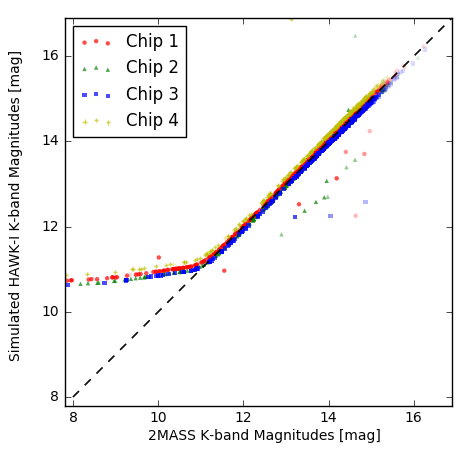
\includegraphics[width=0.45\textwidth]{images/2MASS_vs_HAWKado_inst_mags_single}
    
    \caption{Instrumental K-band magnitudes (Vega) from an observation of M\,4 simulated with SimCADO (SimCADO output) versus K-band magnitudes (Vega) from the 2MASS catalogue (SimCADO input). The one-to-one correlation was to be expected because the brightness levels of the stars in the simulated images were based on the 2MASS catalogue. The cloud of points below the line shows where two stars were close enough together that the pipeline chose the wrong star. It was set up to choose the brightest star within a $1\arcsec$ radius around each coordinate in the 2MASS catalogue. The deviation from the one-to-one line around $K_{s}=11$\m is due to SimCADO reproducing the saturation characteristics of the HAWK-I detector. The effect of the different gain values for the HAWK-I detectors is also visible as the slight offset between the different coloured dots. The instrumental zero-point used was 27.2\m.}
    \label{fig:2mass_hawkado_flux_comparison}

\end{figure}

\begin{figure*}

    \centering
    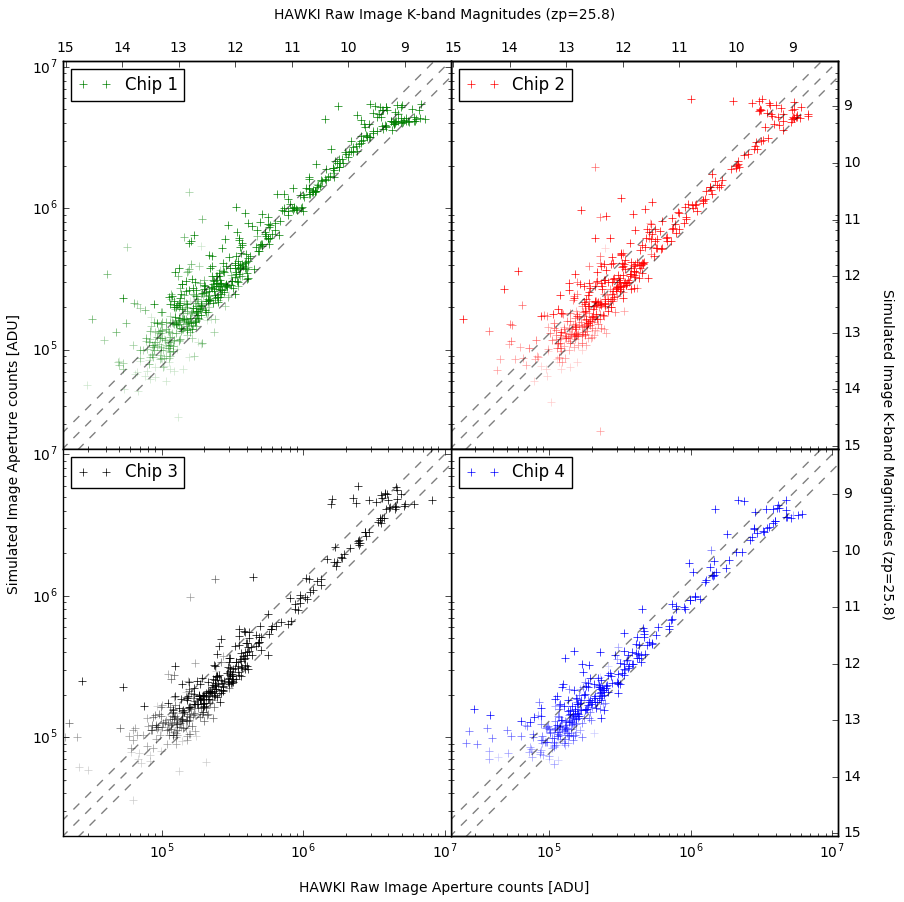
\includegraphics[width=\textwidth]{images/HAWKI_vs_HAWKado_couts_and_mags.png}
    
    \caption{Flux counts from aperture photometry of the stars in the simulated and real Ks-band images of M\,4. Each detector is plotted separately here as they cover different regions of M\,4 and have different gain factors. The strength of the symbols is determined by the photometric quality flag in the 2MASS catalogue. The dashed lines are the $\pm 0.3^\mathrm{m}$, or 30\,\% flux difference intervals. For detectors~1 and~2  more than 75\,\% of stars with A-grade 2MASS photometry fall within these bands. For detectors~3 and~4 this is $>85\,\%$. Approximately 55\,\% of the sources with C-grade or worse 2MASS photometry flags fell outside the $\pm 30\,\%$ bands. When investigating these sources we found a large fraction to be single entries in the 2MASS catalogue, were resolved into multiple stars in the HAWK-I images. Photon statistics only play a role for aperture fluxes on the order of $10^{4}$ counts.}
    \label{fig:HAWKI_hawkado_flux_comparison}
    
\end{figure*}

\begin{figure*}

    \centering
    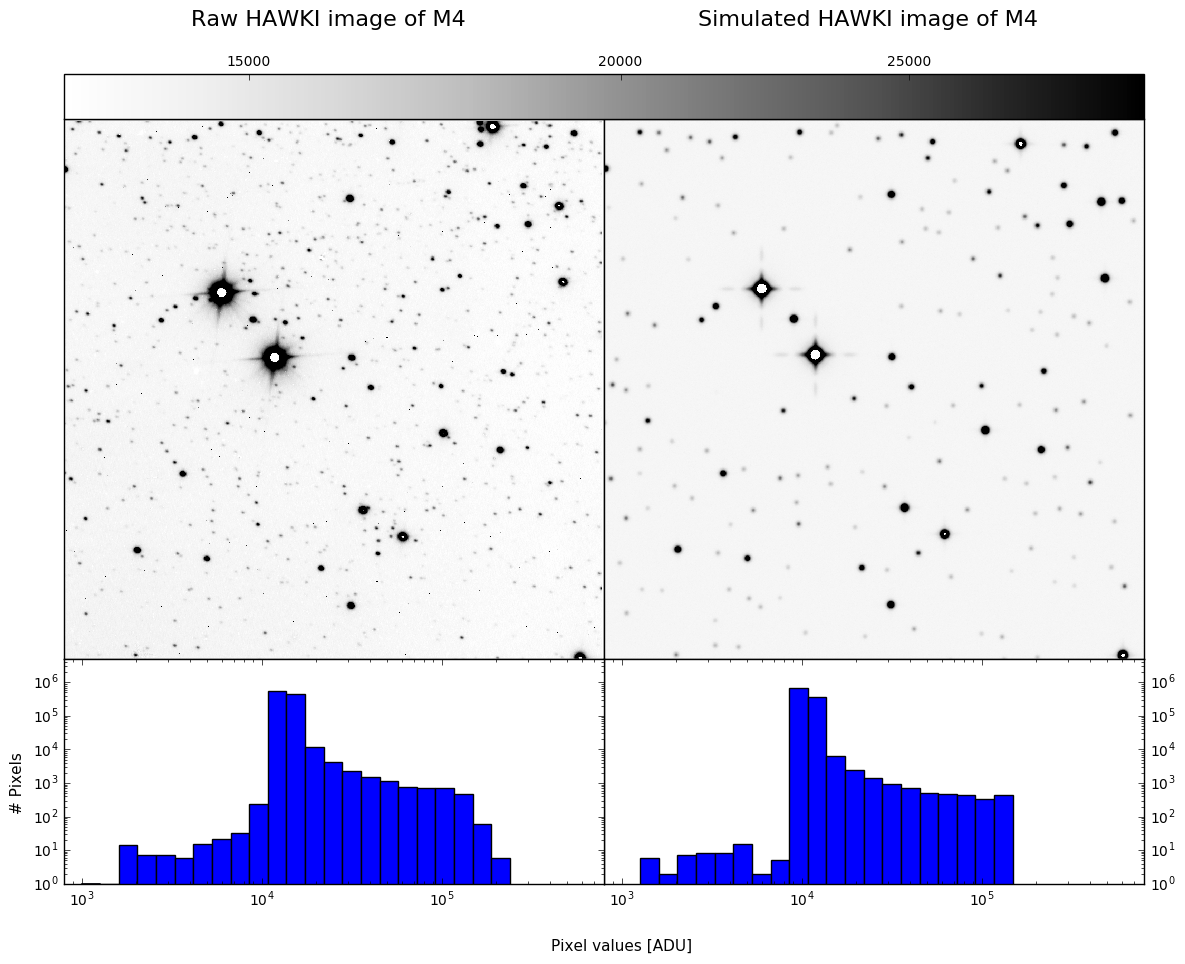
\includegraphics[width=\textwidth]{images/hawki_simcado_side_by_side}
    
    \caption{Top: A comparison of a raw HAWK-I image (left) with a simulated image (right) from SimCADO for the same field near M\,4. The 2MASS point source catalogue was used to populate the simulated images. As such no sources fainter than the 2MASS detection limit were included. Features created by the optical train (e.g.~diffraction spikes) and by the detector (e.g.~saturation) can be seen in both the real and simulated images. The apparent size of the PSF for the brightest stars in the simulated images is smaller than in the real images because SimCADO does not currently model leakage from saturated pixels into neighbouring pixels. Bottom: The distribution of pixel counts for the real (left) and simulated (right) images is given here to illustrate that SimCADO is capable of recreating observations with no ``real world'' input. The discrepancy in the shape of the histogram for pixel counts less that 10\,000 is due to the low resolution custom made linearity curve used by SimCADO. Because of this the saturated pixels in the brightest stars are not perfectly modelled in SimCADO. However, as such pixels are often flagged as unusable by reduction pipelines, refining the accuracy of the linearity curve for SimCADO was deemed less than critical.}
    \label{fig:img_comparison}
    
\end{figure*}


In order to simulate the raw images we generated SimCADO-readable \verb+Source+ objects for the globular clusters M\,4 and NGC\,4147 using the 2MASS sky coordinates and apparent magnitudes of all sources in the respective HAWK-I fields of view. These \verb+Source+-objects were fed into the SimCADO model of HAWK-I and the \verb+Detector+ module was read out. The resulting images were analogues of the raw images generated by the HAWK-I detectors. They contained raw pixel counts in ADUs. We used three-radius fixed aperture photometry to determine the total flux of each star and compared these flux values to the theoretical fluxes calculated from the 2MASS magnitudes. The SimCADO fluxes are in excellent agreement with the 2MASS fluxes. This was to be expected as the 2MASS catalogue provided the input for the SimCADO source model.
Fig.~\ref{fig:2mass_hawkado_flux_comparison} was included to show the reliability of SimCADO when propagating flux through the model of the optical train.
The deviation from the one-to-one line in Fig.~\ref{fig:2mass_hawkado_flux_comparison} is due to SimCADO recreating the linearity and saturation characteristics of the HAWAII-2RG detectors for pixel counts higher than $\sim 100,000$. While it would have been possible to re-run the analysis without a perfectly linear detector response, it was not deemed necessary to illustrate SimCADO's ability to accurately propagate flux through the optical train.

The same fixed aperture photometry method was also applied to the raw HAWK-I images from the archive. Fig.~\ref{fig:HAWKI_hawkado_flux_comparison} shows a comparison between the total aperture flux for stars in a real K-band image of M\,4 (left) and its simulated counterpart (right). There is a good correlation between the fluxes extracted from the two images. For detectors~1 and~2 more than 75\,\% of stars with A-grade 2MASS photometry fall within $\pm0.3$\m of the one-to-one line. For detectors~3 and~4 it is more than 85\,\%. Approximately 55\,\% of the sources with photometry flags C-grade or less fell outside the $\pm0.3$\m zones. Visual inspection of these sources found a large fraction of these to be single 2MASS sources which were resolved into two or more stars in the HAWK-I images. In these cases our photometric pipeline had selected the brightest of the resolved stars in the HAWK-I images and measured its flux. Given that SimCADO had used the 2MASS catalogue as input, in these cases it had simulated single point sources with the combined flux of the resolved sources in the HAWK-I images. This is the primary cause of the scatter seen above the one-to-one line in Fig.~\ref{fig:HAWKI_hawkado_flux_comparison}. Furthermore, as the artificial globular clusters for SimCADO were based on the 2MASS catalogue for M\,4, no sources fainter than the 2MASS detection limit are present in the simulated images. The presence of the fainter background sources, and thus a non-uniform increase in the background flux in the real images further reduced the accuracy of the photometric measurements for sources with magnitudes $K_{s} > 12$\m. In this faint regime ``hot'' or ``dead'' pixels also affected the accuracy of the photometry. As we did not provide SimCADO with the HAWK-I pixel map, the randomized malfunctioning pixels included in the simulated images were not the same as those on the HAWK-I detectors. These pixels are the primary cause of the scatter below the one-to-one line in Fig.~\ref{fig:HAWKI_hawkado_flux_comparison}. Finally, the small but uniform $< 0.1$\m shift in the photometry between detectors was caused by the difference in the detector gain factors \citep{hawki}.

Aside from reproducing the expected stellar fluxes on the detector plane, and more important for predictions relating to MICADO and the ELT, is SimCADO's ability to accurately reproduce the background flux distribution. For the strength of the sky background for the raw archive images, we assumed standard sky background magnitudes as given by \citet{cuby2000}. This assumption was adequate for SimCADO to reproduce the shape of the flux histogram as shown in Fig.~\ref{fig:img_comparison}. It should be noted that the sky background varied between the three sets of archival data. This resulted in background fluxes from SimCADO being $\sim 0.1$\m lower than the backgrounds in the raw J and Ks images from the 2007 observations of M\,4. For the 2015 Ks-band observation the simulated image had a background flux on the order or about $0.4$\m fainter than in the raw HAWK-I image. Given that \citet{moreels08} report that NIR sky backgrounds can vary up to 0.75\m per night, we conclude that this difference is due to the observational conditions\footnote{\url{https://www.eso.org/sci/observing/phase2/ObsConditions.html}}. Further work is currently being done to implement an extended background model so that SimCADO is able to also reliably reproduce the sky background for various combinations of observing conditions such as airmass, seeing and precipitable water vapour. This functionality will use the SkyCalc \citep{skycalc1, skycalc2} API provided by ESO.


\subsection{Differences between the simulated and the real HAWK-I images}

Overall the simulated images of M\,4 and NGC\,4147 compared favourably with the raw observations from the ESO archive. The distribution of pixel flux, background level and noise, total star fluxes and positions, detector noise and saturation, were well reproduced in the simulated images. Magnitudes derived from aperture photometry on the simulated images matched almost perfectly with the 2MASS catalogue for all stars with $J, K_S > 11$\m. When comparing photometry between the simulated and archive images, around two thirds of all the stars measured had flux differences between the images within $\pm 0.3$\m. The scatter seen in Fig.~\ref{fig:HAWKI_hawkado_flux_comparison} is a combination of unresolved sources in the 2MASS catalogue being resolved by HAWK-I, and SimCADO not including the hot pixels on the HAWK-I detectors. Hence this scatter shows that there is a need for a better description of the globular clusters. An extrapolation of the source catalogue down to the detection limit of HAWK-I would be desirable. However, as the coordinates of the fainter sources are unknown, this would likely cause the scatter to increase rather than decrease. With the ELT's ability to detect sources down to $J\approx 29$\m, the prevalence of background sources in this regime will indeed need to be addressed and simulated accurately.

The level of background flux generated by SimCADO for the J and Ks filters is in line with the flux levels returned by the ESO exposure time calculator for HAWK-I. However, only archive J~and Ks~images from 2007 had background levels as low as the ETC and SimCADO. The other two J~and Ks~images had levels 10\,\% and 30\,\% higher. While there is an abundance of information on the weather conditions during the observations, we were unable to find estimates for the measured sky background. We therefore used the standard Paranal background magnitudes for the simulations. As NIR sky background flux levels can vary by up to 0.75\m over the course of a night \citep{moreels08}, we do not see the difference between the simulated and real background fluxes in these images as a major failure of the software. Moreover, dynamic sky background variation is yet another effect that should be added to a future release of SimCADO.

A final caveat for the software verification is that the model of the optical train for UT4/HAWK-I is based on the information available on the ESO website and from the HAWK-I user manual. Despite our due diligence it is possible that some of the data used by SimCADO is inaccurate or not up to date. 

% In order to further test how SimCADO reacts to different sets of observing conditions (airmass, seeing, etc), we submitted a ESO proposal in Period 100 for technical time on HAWK-I. We are still waiting on the completion of the observing run before embarking on a new validation campaign. This should allow us to further increase the accuracy of the simulated images by allowing us to implement each aspect of the atmospheric background separately. 